\documentclass[pra, onecolumn, notitlepage, floats, 11pt]{revtex4-1}

\usepackage[T1]{fontenc}
\usepackage{graphicx}
\usepackage{color}
\usepackage{latexsym,amsmath}
\usepackage{comment}
\usepackage{tabularx}
\usepackage{siunitx}
\usepackage{multirow}
\usepackage{mathtools}
\usepackage{tikz, fp}
\usepackage{wrapfig}
\usepackage{amsfonts}
\usepackage{bbold}
\usepackage[pdftex,colorlinks=true, pdfstartview=FitV, linkcolor=linkcolor, citecolor=linkcolor, urlcolor=linkcolor, hyperindex=true,hyperfigures=true]{hyperref} %hyperlink%
\usepackage{fancyhdr}
\usepackage{inconsolata}
\usepackage{listings}
\usepackage{physics}
\usepackage{datetime}
\usepackage[caption=false]{subfig}
\usepackage{titlesec}

\renewcommand{\figurename}{Figure}
\renewcommand{\tablename}{Table}
\renewcommand{\thetable}{\arabic{table}}

\definecolor{airforceblue}{rgb}{0.36, 0.54, 0.66}  %#5D8AA8
\definecolor{cobalt}{rgb}{0.0, 0.28, 0.67}         %#0047AB
\definecolor{coolblack}{rgb}{0.0, 0.18, 0.39}      %#002E63
\definecolor{dartmouthgreen}{rgb}{0.05, 0.5, 0.06} %#00693E
\definecolor{mydmg}{rgb}{0.05, 0.5, 0.06}          %#00693E
\definecolor{lava}{rgb}{0.81, 0.06, 0.13}          %#CF1020
\definecolor{myred}{rgb}{0.81, 0.06, 0.13}         %#CF1020
% move section headings to left
% \sffamily
% \scshape
%\titleformat{\section}{\raggedright\sffamily\bfseries\fontsize{13pt}{13}\selectfont}{\arabic{section}}{1em}{\MakeUppercase}
\titleformat{\section}{\raggedright\bfseries\scshape\fontsize{13pt}{13}\selectfont}{\color{cobalt}\arabic{section}}{1em}{\color{cobalt}}
\titleformat{\subsection}{\raggedright\bfseries\scshape\fontsize{12pt}{12}\selectfont}{{\color{cobalt}\arabic{section}.\arabic{subsection}}}{1em}{\color{cobalt}}
\renewcommand{\thesection}{\arabic{section}}
\renewcommand{\thesubsection}{\arabic{subsection}}
\renewcommand{\thesubsubsection}{\arabic{subsubsection}}
\makeatletter
\renewcommand{\p@subsection}{\thesection.}
\renewcommand{\p@subsubsection}{\thesection.\thesubsection.}
\makeatother


\linespread{0.956}

\DeclarePairedDelimiter\ceil{\lceil}{\rceil}
\DeclarePairedDelimiter\floor{\lfloor}{\rfloor}

\definecolor{linkcolor}{rgb}{0,0,0.65}
\definecolor{shadecolor}{rgb}{0.95, 0.95, 0.95}
\definecolor{mygreen}{rgb}{0,0.6,0}
\definecolor{mygray}{rgb}{0.5,0.5,0.5}
\definecolor{mymauve}{rgb}{0.58,0,0.82}
\lstdefinestyle{fortran}
{
    backgroundcolor=\color{shadecolor},       % background color
    basicstyle=\ttfamily\scriptsize,          % the size of the fonts that are used for the code
    breakatwhitespace=false,                  % sets if automatic breaks should only happen at whitespace
    breaklines=false,                         % sets automatic line breaking
    captionpos=b,                             % sets the caption-position to bottom
    commentstyle=\color{mygreen},             % comment style
    extendedchars=true,                       % lets you use non-ASCII characters; for 8-bits encodings only, does not work with UTF-8
    keepspaces=true,                          % keeps spaces in text, useful for keeping indentation of code (possibly needs columns=flexible)
    keywordstyle=\bfseries\color{blue},       % keyword style
    language=[95]Fortran,                     % the language of the code
    numbers=left,                             % where to put the line-numbers; possible values are (none, left, right)
    numbersep=5pt,                            % how far the line-numbers are from the code
    numberstyle=\tiny\color{mygray},          % the style that is used for the line-numbers
    rulecolor=\color{black},                  % if not set, the frame-color may be changed on line-breaks within not-black text (e.g. comments (green here))
    showspaces=false,                         % show spaces everywhere adding particular underscores; it overrides 'showstringspaces'
    showstringspaces=false,                   % underline spaces within strings only
    showtabs=false,                           % show tabs within strings adding particular underscores
    stepnumber=1,                             % the step between two line-numbers. If it's 1, each line will be numbered
    stringstyle=\color{mymauve},              % string literal style
    tabsize=4,                                % sets default tabsize to 4 spaces
    title=\lstname                            % show the filename of files
}

\lstdefinestyle{python}
{
    backgroundcolor=\color{shadecolor},       % background color
    basicstyle=\ttfamily\scriptsize,          % the size of the fonts that are used for the code
    breakatwhitespace=false,                  % sets if automatic breaks should only happen at whitespace
    breaklines=false,                         % sets automatic line breaking
    captionpos=b,                             % sets the caption-position to bottom
    commentstyle=\color{mygreen},             % comment style
    extendedchars=true,                       % lets you use non-ASCII characters; for 8-bits encodings only, does not work with UTF-8
    keepspaces=true,                          % keeps spaces in text, useful for keeping indentation of code (possibly needs columns=flexible)
    keywordstyle=\bfseries\color{blue},       % keyword style
    language=Python,                          % the language of the code
    numbers=left,                             % where to put the line-numbers; possible values are (none, left, right)
    numbersep=5pt,                            % how far the line-numbers are from the code
    numberstyle=\tiny\color{mygray},          % the style that is used for the line-numbers
    rulecolor=\color{black},                  % if not set, the frame-color may be changed on line-breaks within not-black text (e.g. comments (green here))
    showspaces=false,                         % show spaces everywhere adding particular underscores; it overrides 'showstringspaces'
    showstringspaces=false,                   % underline spaces within strings only
    showtabs=false,                           % show tabs within strings adding particular underscores
    stepnumber=1,                             % the step between two line-numbers. If it's 1, each line will be numbered
    stringstyle=\color{mymauve},              % string literal style
    tabsize=4,                                % sets default tabsize to 4 spaces
    title=\lstname                            % show the filename of files
}

\lstdefinestyle{bash}
{
    backgroundcolor=\color{shadecolor},       % background color
    basicstyle=\ttfamily\scriptsize,          % the size of the fonts that are used for the code
    breakatwhitespace=false,                  % sets if automatic breaks should only happen at whitespace
    breaklines=false,                         % sets automatic line breaking
    captionpos=b,                             % sets the caption-position to bottom
    commentstyle=\color{mygreen},             % comment style
    extendedchars=true,                       % lets you use non-ASCII characters; for 8-bits encodings only, does not work with UTF-8
    keepspaces=true,                          % keeps spaces in text, useful for keeping indentation of code (possibly needs columns=flexible)
    keywordstyle=\bfseries\color{blue},       % keyword style
    language=bash,                            % the language of the code
    numbers=left,                             % where to put the line-numbers; possible values are (none, left, right)
    numbersep=5pt,                            % how far the line-numbers are from the code
    numberstyle=\tiny\color{mygray},          % the style that is used for the line-numbers
    rulecolor=\color{black},                  % if not set, the frame-color may be changed on line-breaks within not-black text (e.g. comments (green here))
    showspaces=false,                         % show spaces everywhere adding particular underscores; it overrides 'showstringspaces'
    showstringspaces=false,                   % underline spaces within strings only
    showtabs=false,                           % show tabs within strings adding particular underscores
    stepnumber=1,                             % the step between two line-numbers. If it's 1, each line will be numbered
    stringstyle=\color{mymauve},              % string literal style
    tabsize=4,                                % sets default tabsize to 4 spaces
    title=\lstname                            % show the filename of files
}

\makeatletter
\newcommand{\srcsize}{\@setfontsize{\srcsize}{5pt}{5pt}}
\makeatother


\pagestyle{fancy}
\fancyhf{}
\fancyhead[L]{Rocco Ardino (Mat. 1231629)}
\fancyhead[R]{\bf\thepage}
\fancyfoot[L]{\textsc{report}: Week 10}
\fancyfoot[R]{\today}
\renewcommand{\headrulewidth}{0.1pt}
\renewcommand{\footrulewidth}{0.1pt}

\newcommand{\codebold}[2][cobalt]{\texttt{\bfseries {\color{#1}#2}}}
\newcommand{\code}[2][black]{\color{#1}\texttt{#2}}
\newcommand{\codefunctionbold}[2]{\texttt{\bfseries {\color{cobalt}#1}({\color{lava}#2})}}
\newcommand{\codefunction}[2]{\texttt{#1(#2})}










\begin{document}

\title{Quantum Information and Computing 2020/21\\Week 10 report}

\author{Rocco Ardino}

\date{\today}





\begin{abstract}
    In this work we deal with the monodimensional Ising model Hamiltonian and with the Renormalization Group techniques for the problem. In particular, starting from the code for the last week assignment, we implement the RSRG algorithm to find the ground state of the Hamiltonian with an improved accuracy. For the purpose, we exploit the Lapack library for the diagonalization and to find the eigenvalues. Lastly, the ground state energy is plotted with respect to the interaction strength parameter and the result is confronted with the mean field solution.
\end{abstract}

\maketitle





\section{Theory}
The monodimensional Ising model describes a linear chain of \( N \) spins under the action of a magnetic field. The Hamiltonian describing such a system reads:
\begin{equation}
    H
    =
    \lambda \sum_{i=1}^{N} \sigma_{i}^{z} + \sum_{i=1}^{N-1} \sigma_{i}^{x} \sigma_{i+1}^{x}
    \quad ,
    \label{eq:10_T_1}
\end{equation}
where \( \lambda \) is the interaction strength and the \( \sigma \)'s are the Pauli matrices, for which the following notation is employed:
\begin{align}
    \sigma_{i}^{z}
    &=
        \mathbb{1}_{1} \otimes \cdots \mathbb{1}_{i-1} \otimes \sigma_{i}^{z} \otimes \mathbb{1}_{i+1} \otimes \cdots \mathbb{1}_{N}    \\
    \sigma_{i}^{x} \sigma_{i+1}^{x}
    &=
        \mathbb{1}_{1} \otimes \cdots \mathbb{1}_{i-1} \otimes \sigma_{i}^{x} \otimes \sigma_{i+1}^{x} \otimes \mathbb{1}_{i+2} \otimes \cdots \mathbb{1}_{N}
        \quad .
\end{align}

In order to get the ground state of \( H \) with good accuracy, we can exploit the Real Space Renormalization Group (RSRG) algorithm. This is based on the hypothesis that the ground state of a composite system is a sum of the low energy states of the subsystem. Its application goes through the following steps:
\begin{itemize}
    \setlength\itemsep{-3pt}
    \item we consider the Hamiltonian \( H_{N} \) of a subsystem, whose eigenvalues and eigenvectors are known;
    \item we double this system into a system of \( 2N \) particles and form its Hamiltonian:
    \begin{equation}
        H_{2N}
        =
        H_{N} \otimes \mathbb{1}^{\otimes N}_{2} + \mathbb{1}^{\otimes N}_{2} \otimes H_{N} + H_{\mathrm{int}}
        \quad ,
        \label{eq:10_T_2}
    \end{equation}
    where \( H_{\mathrm{int}} \) can be separated in the two components acting on the two subsystems of \( N \) particles, namely \( H_{L} \) and \( H_{R} \), and it reads:
    \begin{equation}
        H_{\mathrm{int}}
        =
        H_{L} \otimes H_{R}
        \quad ;
        \label{eq:10_T_3}
    \end{equation}
    \item we disagonalize \( H_{2N} \) and project the first \( N \) eigenvectors with lowest eigenvalue into the \( N^{2} \times N \) matrix \( P \);
    \item we compute the new Hamiltonian matrix \( H \), and the new left and right interaction matrices \( H_{L} \) and \( H_{R} \):
    \begin{subequations}
        \begin{align}
            H_{N} &= P^{\dag} H_{2N} P                  \\
            H_{L} &= P^{\dag} H_{L}  P  \quad\quad ;    \\
            H_{R} &= P^{\dag} H_{R}  P
        \end{align}
        \label{eq:10_T_4}
    \end{subequations}
    \item we iterate the previous steps with the new \( H \), \( H_{L} \) and \( H_{R} \), until we reach a desired number of iterations \( n_{\mathrm{it}} \), so that the energy density will be given by:
    \begin{equation}
        \rho_{\mathrm{gs}}
        =
        \frac{E_{\mathrm{gs}}}{N \cdot 2^{n_{\mathrm{it}}}}
        \quad .
        \label{eq:10_T_5}
    \end{equation}
\end{itemize}

After applying the RSRG algorithm, the results obtained should be compared with the mean field solution, which reads:
\begin{equation}
    E_{\mathrm{gs}}^{\mathrm{mf}}(\lambda)
    =
    \begin{cases}
        - 1 - \frac{\lambda^{2}}{4}     &   \lambda \in [-2,2]  \\
        - \abs{\lambda}                 &   \lambda \notin [-2,2]
    \end{cases}
    \label{eq:10_T_6}
\end{equation}
In particular, we expect that the ground state energy in the non-interacting case, namely for \( \lambda = 0 \), should be equal to \( -1 \).





\section{Code Development}
For this work, the module \codebold{ising\_utils} from the previous assignment has been updated and it contains several functions and subroutines for multiple purposes. In particular:
\vspace{-5pt}
\begin{itemize}%[nolistsep]
    \setlength\itemsep{-3pt}
    \item \codefunctionbold{ising\_tensor\_prod}{mat1,mat2}, for executing the tensor product of the two input matrices \code{mat1} and \code{mat2};
    \item \codefunctionbold{ising\_identity}{N}, for instantiating the identity matrix for \code{N} spins, so of dimensions \( 2^{\code{N}} \times 2^{\code{N}} \);
    \item \codefunctionbold{ising\_hmat\_init}{N,L}, for initializing the Ising Hamiltonian for \code{N} spins and an interaction strength parameter \code{L};
    \item \codefunctionbold{ising\_hmat\_diag}{hmat,eigvc,eigvl}, for diagonalizing the Ising Hamiltonian and returning both the eigenfunctions (in the \code{eigvc} input variable) and the eigenvalues (in \code{eigvl});
    \item \codefunctionbold{ising\_hmat\_rsrg}{hmat,hmat\_L,hmat\_R,N,L}, for applying a single iteration of the RSRG algorithm, with \( \code{hmat} = H_{N} \), \( \code{hmat\_L} = H_{L} \) and \( \code{hmat\_R} = H_{R} \);
    \item \codefunctionbold{ising\_print\_hmat\_std}{hmat,formatted}, for printing the Ising Hamiltonian matrix entries on standard output and in a formatted way, if specified.
\end{itemize}

Moreover, another module, namely \codebold{cmdline}, is implemented to have a command-line argument parser and for default arguments handling. In particular, we explain the new core functionalities of both the modules in the following subsections. Note that the implementation of \code{ising\_tensor\_prod}, \code{ising\_hmat\_init} and \code{ising\_hmat\_diag} has already been treated in the previous week report, so we will not discuss about it for brevity.



\subsection{RSRG algorithm implementation}
The code to apply a single iteration of RSRG algorithm is showed in Listing \ref{lst:10_C_SS_1_1}. Note how the input matrices \( H_{2N} \), \( H_{L} \) and \( H_{R} \) are updated and stored again in the same input variable.

\begin{lstlisting}[
    style=fortran,
    frame=single,
    label={lst:10_C_SS_1_1},
    caption={Implementation of the single iteration of the RSRG algorithm.}
]
subroutine ising_hmat_rsrg(hmat, hmat_L, hmat_R, N)
    ! input arguments
    complex(8), dimension(:,:) :: hmat, hmat_L, hmat_R    ! input arguments
    integer(4) :: N                                       ! input arguments

    complex(8), dimension(2**(2*N), 2**(2*N)) :: hmat_2N, hmat_2N_eigvc
    complex(8), dimension(2**(2*N), 2**(2*N)) :: hmat_L_int, hmat_R_int
    complex(8), dimension(2**(2*N), 2**(N)  ) :: hmat_P
    complex(8), dimension(2**(N)  , 2**(2*N)) :: hmat_PA
    real(8),    dimension(2**(2*N))           :: hmat_2N_eigvl

    ! initialize 1+2 Hamiltonian
    hmat_2N    = ising_tensor_prod(hmat, ising_identity(N)) + &
                 ising_tensor_prod(ising_identity(N), hmat) + &
                 ising_tensor_prod(hmat_L, hmat_R)
    ! diagonalize 1+2 Hamiltonian
    call ising_hmat_diag(hmat_2N, hmat_2N_eigvc, hmat_2N_eigvl)
    ! project Hamiltonian
    hmat_P     = hmat_2N_eigvc(:,:2**N)
    hmat_PA    = TRANSPOSE(CONJG(hmat_P))
    ! update Hamiltonian
    hmat       = MATMUL(MATMUL(hmat_PA, hmat_2N), hmat_P)
    ! update hmat_L and hmat_R
    hmat_L_int = ising_tensor_prod(hmat_L, ising_identity(N))
    hmat_R_int = ising_tensor_prod(ising_identity(N), hmat_R)
    hmat_L     = MATMUL(MATMUL(hmat_PA, hmat_L_int), hmat_P)
    hmat_R     = MATMUL(MATMUL(hmat_PA, hmat_R_int), hmat_P)
end subroutine ising_hmat_rsrg
\end{lstlisting}



\subsection{Main program}
Lastly, all the functions described before are employed in a main program, in which a command-line argument parser is implemented in order to obtain an easier handling of the parameters of the simulation. Moreover, this functionality is also capable of giving default values to the arguments when they are not given.
To make the program more user-friendly, a \code{-h} help option has been added and in the beginning of the execution all the arguments given are printed along with a flag: \codebold[red]{F} if a value is given for it, \codebold[dartmouthgreen]{T} if default is taken. An example of this functionality and of the way to start the program is showed in Listing \ref{lst:10_C_SS_2_1}. A complete list of the options is given in Table \ref{tab:10_C_SS_2_1}.

\begin{table}[!h]
\begin{minipage}[t]{0.48\textwidth}
    \raisebox{-\height}{
    {\footnotesize
    \begin{tabular}{cccc}
        \toprule
        Arg option    &   Arg name        &   Arg meaning   &   Default     \\
        \colrule
        \code{-N}    &   \code{nspins}      &   \( N \)                 &   \(  2 \)    \\
        \code{-L}    &   \code{lambda}      &   \( \lambda \)           &   \(  1 \)    \\
        \code{-I}    &   \code{iterations}  &   \( n_{\mathrm{it}} \)   &   \( 10 \)    \\
        \code{-h}    &   \code{help}        &   print help              &               \\
        \botrule
    \end{tabular}
    }}
    \caption{Command-line arguments of the program.}
    \label{tab:10_C_SS_2_1}
\end{minipage}
\hfill
\begin{minipage}[t]{0.48\textwidth}
\begin{lstlisting}[
    style=bash,
    frame=single,
    escapechar=!,
    label={lst:10_C_SS_2_1},
    caption={Example of launch and user interface.}
]
!{\bfseries\color{dartmouthgreen}\$}! !{\bfseries\color{cobalt}./10.o}! !{\bfseries\color{lava}-L}! 0 !{\bfseries\color{lava}-I}! 100

Running with the following cmdline options:

N =	       2	default [T/F]: !{\bfseries\color{dartmouthgreen}T}!
L =	     0.0   	default [T/F]: !{\bfseries\color{red}F}!
I =	     100	default [T/F]: !{\bfseries\color{red}F}!

-1.0000000000000324
\end{lstlisting}
\end{minipage}
\end{table}

After the parser, if no exception is found, a subroutine with the main execution is run, which in order:
\begin{itemize}
    \setlength\itemsep{-3pt}
    \item initializes the Ising Hamiltonian \( H \) for \( N \) spins and for an interaction strength \( \lambda \);
    \item initializes \( H_{L} \) and \( H_{R} \);
    \item applies \( n_{\mathrm{it}} \) iterations of the RSRG algorithm;
    \item prints the final result for the ground state energy on the standard output.
\end{itemize}
The implementation of these steps is showed in Listing \ref{lst:10_C_SS_2_2}. Last but not least, the program must be compiled with the flag \code{-ffree-line-length-0}.

\begin{lstlisting}[
    style=fortran,
    frame=single,
    label={lst:10_C_SS_2_2},
    caption={Core operations performed in the main program.}
]
hmat   = ising_hmat_init(N, L)                          ! initialization of H
hmat_L = ising_tensor_prod(ising_identity(N-1), s_x)    ! initialization of H_{L}
hmat_R = ising_tensor_prod(s_x, ising_identity(N-1))    ! initialization of H_{R}

do ii=1,I
    hmat   = hmat   * 0.5d0                             ! rescale to avoid overflow
    hmat_L = hmat_L * SQRT(0.5d0)                       ! rescale to avoid overflow
    hmat_R = hmat_R * SQRT(0.5d0)                       ! rescale to avoid overflow

    call ising_hmat_rsrg(hmat, hmat_L, hmat_R, N)       ! apply iterations of RSRG algorithm
end do

call ising_hmat_diag(hmat, eigvc, eigvl)                ! final diagonalization

write(*, "(g0)") eigvl(1) / N                           ! print results on stdout
\end{lstlisting}

In order to automatize every step for different parameters for \( N \) and \( \lambda \), a Python script is employed to run multiple batch executions for different sets of input parameters. Then, the results are stored in appropriately labelled files.





\section{Results}
The main program is run requiring to print the ground state energy after \( n_{\mathrm{it}} = 100 \). Therefore, we are simulating a system of \( N \cdot 2^{n_{\mathrm{it}}+1} \) spins. In particular, we choose \( N = 2, 3, 4 \) and \( \lambda \in [-3,3] \).
The results obtained for this set of parameters are plotted through a Gnuplot script and they are showed in Figure \ref{fig:10_R_1} along with the mean field solution.

\begin{figure*}[!h]
    \centering
    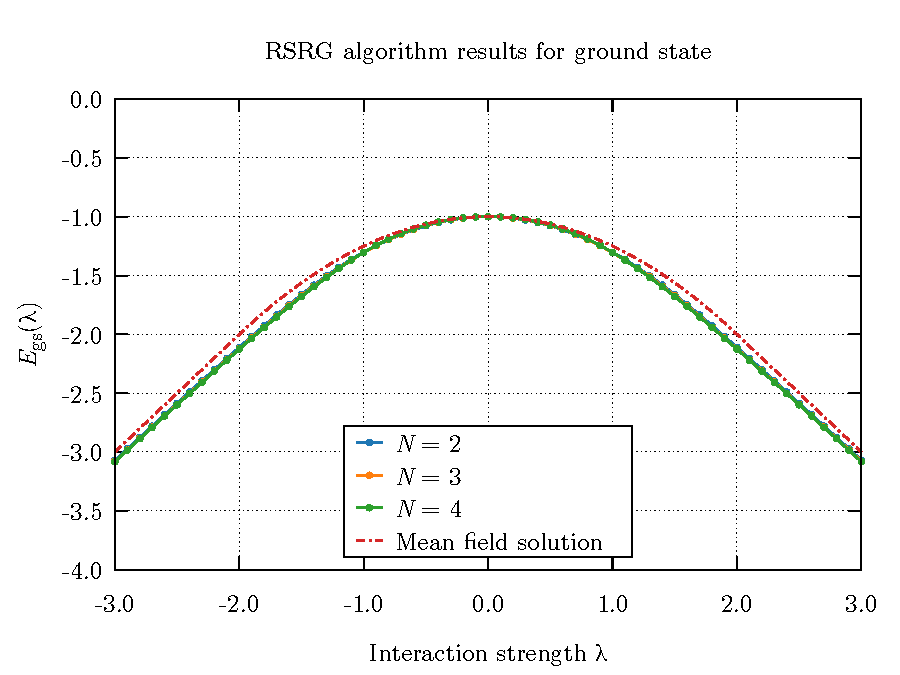
\includegraphics[width=0.75\textwidth]{images/ising_RSRG_100_I.pdf}
    \caption{Ground state energy of Ising Hamiltonian depending on the interaction strength \( \lambda \) and for \( N = 2, 3, 4 \), and comparison with the mean field solution.}
    \label{fig:10_R_1}
\end{figure*}

What we can observe is that the ground state energy for the non-interacting case, namely for \( \lambda = 0 \), is \( -1 \), as predicted by the mean field solution.
We can also observe how the numerical solution obtained from the RSRG algorithm is practically the same for every value of \( N \) tested and that these are in agreement with the mean field solution only for small values of \( \lambda \). When \( \lambda \) is increased, a discrepancy appears as a constant shift in the energy.





\section{Self-evaluation}
In this work we have successfully tackled the problem of one-dimensional Ising model simulation using the RSRG algorithm. The simulations showed in the results have been run for a number of iterations \( n_{\mathrm{it}} = 100 \) and for several values of \( N \), showing stable and accurate results.
These are compared with the mean field solution, showing a discrepancy for higher values of \( \lambda \). Further studies should be done in this direction, implementing the Infinite Density Matrix Renormalization Group (DMRG) algorithm and comparing again the results.

\end{document}
